% Options for packages loaded elsewhere
% Options for packages loaded elsewhere
\PassOptionsToPackage{unicode}{hyperref}
\PassOptionsToPackage{hyphens}{url}
\PassOptionsToPackage{dvipsnames,svgnames,x11names}{xcolor}
%
\documentclass[
  11pt,
]{article}
\usepackage{xcolor}
\usepackage[margin = 1in]{geometry}
\usepackage{amsmath,amssymb}
\setcounter{secnumdepth}{-\maxdimen} % remove section numbering
\usepackage{iftex}
\ifPDFTeX
  \usepackage[T1]{fontenc}
  \usepackage[utf8]{inputenc}
  \usepackage{textcomp} % provide euro and other symbols
\else % if luatex or xetex
  \usepackage{unicode-math} % this also loads fontspec
  \defaultfontfeatures{Scale=MatchLowercase}
  \defaultfontfeatures[\rmfamily]{Ligatures=TeX,Scale=1}
\fi
\usepackage{lmodern}
\ifPDFTeX\else
  % xetex/luatex font selection
  \setmainfont[]{Palatino}
  \setmathfont[]{STIX Two Math}
\fi
% Use upquote if available, for straight quotes in verbatim environments
\IfFileExists{upquote.sty}{\usepackage{upquote}}{}
\IfFileExists{microtype.sty}{% use microtype if available
  \usepackage[]{microtype}
  \UseMicrotypeSet[protrusion]{basicmath} % disable protrusion for tt fonts
}{}
\usepackage{setspace}
\makeatletter
\@ifundefined{KOMAClassName}{% if non-KOMA class
  \IfFileExists{parskip.sty}{%
    \usepackage{parskip}
  }{% else
    \setlength{\parindent}{0pt}
    \setlength{\parskip}{6pt plus 2pt minus 1pt}}
}{% if KOMA class
  \KOMAoptions{parskip=half}}
\makeatother


\usepackage{longtable,booktabs,array}
\usepackage{calc} % for calculating minipage widths
% Correct order of tables after \paragraph or \subparagraph
\usepackage{etoolbox}
\makeatletter
\patchcmd\longtable{\par}{\if@noskipsec\mbox{}\fi\par}{}{}
\makeatother
% Allow footnotes in longtable head/foot
\IfFileExists{footnotehyper.sty}{\usepackage{footnotehyper}}{\usepackage{footnote}}
\makesavenoteenv{longtable}
\usepackage{graphicx}
\makeatletter
\newsavebox\pandoc@box
\newcommand*\pandocbounded[1]{% scales image to fit in text height/width
  \sbox\pandoc@box{#1}%
  \Gscale@div\@tempa{\textheight}{\dimexpr\ht\pandoc@box+\dp\pandoc@box\relax}%
  \Gscale@div\@tempb{\linewidth}{\wd\pandoc@box}%
  \ifdim\@tempb\p@<\@tempa\p@\let\@tempa\@tempb\fi% select the smaller of both
  \ifdim\@tempa\p@<\p@\scalebox{\@tempa}{\usebox\pandoc@box}%
  \else\usebox{\pandoc@box}%
  \fi%
}
% Set default figure placement to htbp
\def\fps@figure{htbp}
\makeatother


% definitions for citeproc citations
\NewDocumentCommand\citeproctext{}{}
\NewDocumentCommand\citeproc{mm}{%
  \begingroup\def\citeproctext{#2}\cite{#1}\endgroup}
\makeatletter
 % allow citations to break across lines
 \let\@cite@ofmt\@firstofone
 % avoid brackets around text for \cite:
 \def\@biblabel#1{}
 \def\@cite#1#2{{#1\if@tempswa , #2\fi}}
\makeatother
\newlength{\cslhangindent}
\setlength{\cslhangindent}{1.5em}
\newlength{\csllabelwidth}
\setlength{\csllabelwidth}{3em}
\newenvironment{CSLReferences}[2] % #1 hanging-indent, #2 entry-spacing
 {\begin{list}{}{%
  \setlength{\itemindent}{0pt}
  \setlength{\leftmargin}{0pt}
  \setlength{\parsep}{0pt}
  % turn on hanging indent if param 1 is 1
  \ifodd #1
   \setlength{\leftmargin}{\cslhangindent}
   \setlength{\itemindent}{-1\cslhangindent}
  \fi
  % set entry spacing
  \setlength{\itemsep}{#2\baselineskip}}}
 {\end{list}}
\usepackage{calc}
\newcommand{\CSLBlock}[1]{\hfill\break\parbox[t]{\linewidth}{\strut\ignorespaces#1\strut}}
\newcommand{\CSLLeftMargin}[1]{\parbox[t]{\csllabelwidth}{\strut#1\strut}}
\newcommand{\CSLRightInline}[1]{\parbox[t]{\linewidth - \csllabelwidth}{\strut#1\strut}}
\newcommand{\CSLIndent}[1]{\hspace{\cslhangindent}#1}



\setlength{\emergencystretch}{3em} % prevent overfull lines

\providecommand{\tightlist}{%
  \setlength{\itemsep}{0pt}\setlength{\parskip}{0pt}}



 


%%% Setup for frontmatter, spacing, and colors %%%

\usepackage{orcidlink} % for Orchid ID

% set the geometry of the document
\usepackage{indentfirst} % indent first para
\setlength{\parindent}{0.5in} % set indent length
\setlength{\parskip}{0em} % no extra space between paras

% set spacing of section titles
\usepackage{titlesec} % to set spacing of section titles
\titlespacing\section{0pt}{1\baselineskip}{0.3\baselineskip}
\titlespacing\subsection{0pt}{0.75\baselineskip}{0.2\baselineskip}
\titlespacing\subsubsection{0pt}{0.6\baselineskip}{0.15\baselineskip}

%%% Figures and Tables %%%

% captions 
\usepackage{caption}
\captionsetup{
  %captionskip = 0pt,   % eliminate space bw capiton and figure
  %font = bf,            % make the font of the entire caption bold
  %font = footnotesize,         % make font of entire caption smaller
  justification = raggedright, % left justify the caption 
  singlelinecheck = false,     % apply justification even for single-line captions
  labelfont = bf               % make the caption label bold
}
\setlength{\abovecaptionskip}{10pt} % Adjust the space above the caption

% for rotating figures and tables
\usepackage{rotating}
\usepackage{pdflscape}
\usepackage{float}         % enables [H] float placement specifier
\usepackage{placeins}     % enables \FloatBarrier
\floatplacement{table}{H} % all tables placed exactly where they appear in source

%%% Abstract %%%

\usepackage{abstract}
\renewcommand{\abstractname}{ABSTRACT\vspace{.5em}}
\renewcommand{\abstractnamefont}{\normalfont\bfseries}
\renewcommand{\abstracttextfont}{\normalsize}
\setlength{\absleftindent}{\parindent}
\setlength{\absrightindent}{\parindent}

%% Title %%%

\usepackage{titling}
%\setlength{\droptitle}{3em}
\pretitle{\par\vskip 3em\begin{center}\LARGE\bfseries}
\posttitle{\par\end{center}\vspace{2\baselineskip}}

%%% New commands %%%

% Keywords
\providecommand{\keywords}[1]{\textbf{\textit{Keywords---}}#1}

% Keywords
\providecommand{\fundinginfo}[1]{\textbf{\textit{Funding: }}#1}

% Word count
\providecommand{\wordcount}[1]{\textbf{Word Count: }#1}

% Conflicts
\providecommand{\conflicts}[1]{\textbf{\textit{Conflicts of Interest: }}#1}

% Command for a note at the top of the first page describing the publication
% status of the paper.
\newcommand{\published}[1]{%
   \gdef\puB{#1}}
   \newcommand{\puB}{}
   \renewcommand{\maketitlehooka}{%
       \par\noindent\footnotesize\sffamily\puB}
\makeatletter
\@ifpackageloaded{caption}{}{\usepackage{caption}}
\AtBeginDocument{%
\ifdefined\contentsname
  \renewcommand*\contentsname{Table of contents}
\else
  \newcommand\contentsname{Table of contents}
\fi
\ifdefined\listfigurename
  \renewcommand*\listfigurename{List of Figures}
\else
  \newcommand\listfigurename{List of Figures}
\fi
\ifdefined\listtablename
  \renewcommand*\listtablename{List of Tables}
\else
  \newcommand\listtablename{List of Tables}
\fi
\ifdefined\figurename
  \renewcommand*\figurename{Figure}
\else
  \newcommand\figurename{Figure}
\fi
\ifdefined\tablename
  \renewcommand*\tablename{Table}
\else
  \newcommand\tablename{Table}
\fi
}
\@ifpackageloaded{float}{}{\usepackage{float}}
\floatstyle{ruled}
\@ifundefined{c@chapter}{\newfloat{codelisting}{h}{lop}}{\newfloat{codelisting}{h}{lop}[chapter]}
\floatname{codelisting}{Listing}
\newcommand*\listoflistings{\listof{codelisting}{List of Listings}}
\makeatother
\makeatletter
\makeatother
\makeatletter
\@ifpackageloaded{caption}{}{\usepackage{caption}}
\@ifpackageloaded{subcaption}{}{\usepackage{subcaption}}
\makeatother
\usepackage{bookmark}
\IfFileExists{xurl.sty}{\usepackage{xurl}}{} % add URL line breaks if available
\urlstyle{same}
\hypersetup{
  pdftitle={The Spatial Diffusion of Labor Strikes},
  pdfauthor={Emmanuel Teitelbaum},
  pdfkeywords={labor strikes, strike diffusion, spatial
contagion, subnational panel data, GDELT, collective action},
  colorlinks=true,
  linkcolor={Blue4},
  filecolor={Maroon},
  citecolor={Blue4},
  urlcolor={Blue4},
  pdfcreator={LaTeX via pandoc}}


%% Main title %%

\title{The Spatial Diffusion of Labor Strikes\thanks{Early draft. Please
do not circulate or cite.}}

%% Subtitle %%

\usepackage{etoolbox}
\makeatletter
\providecommand{\subtitle}[1]{% add subtitle to \maketitle
  \apptocmd{\@title}{\par {\vskip 0.25em \large #1 \par}}{}{}
}
\makeatother
\subtitle{Evidence from Global Subnational Event Data}

%% Author info %%

  \author{Emmanuel Teitelbaum
~\orcidlink{0000-0001-7089-0588}
\\George Washington University
\\Department of Political Science
\\\href{mailto:ejt@gwu.edu}{ejt@gwu.edu}
 }

% Omit the date since the \published command does that
\date{}  % blank date

\usepackage{url}
\urlstyle{same}
\begin{document}
%%% Title Section %%%

\newgeometry{top=0.5in, bottom=1in, left=1in, right=1in}

\published{\textbf{2026-03-20} \qquad Prepared for the APSA Labor
Group's Comparative Politics Workshop. \\ {\scriptsize Access the code,
data, and analysis at
\url{https://github.com/eteitelbaum/gdelt-strikes.git}}}

\vspace{0.25in}

\maketitle

\vspace{0.25in}

%%% Abstract %%%

\begin{abstract}
\noindent            %eliminate indent in abstract
Theoretical accounts of labor mobilization emphasize demonstration
effects and geographic diffusion, yet quantitative research rarely
employs identification strategies that distinguish genuine contagion
from common shocks. I examine the spatial structure of strike diffusion
using a subnational panel of first-level administrative units observed
weekly from 2015 to 2025, drawing on 11,503 validated strike events
geocoded from GDELT to ADM1 boundaries. Two-way fixed effects models
with unit and country-by-week fixed effects absorb both time-invariant
confounders and national-level shocks. I find that regions with a
striking neighbor are 3.5 times more likely to strike in the raw data,
but this association fully disappears once national dynamics are
controlled. Decomposing geographic and national channels explicitly
reveals large national contagion effects, while geographic neighbor
exposure adds nothing once country-level activity is controlled.
Exploratory evidence from V-Dem suggests that freedom of expression
amplifies national waves while freedom of association strengthens
geographic transmission. These findings suggest that strike contagion,
unlike civil conflict spillovers, operates at the national rather than
geographic level, and that institutional factors such as freedom of
expression and association may shape the structure of national waves
rather than geographic diffusion per se.
\end{abstract}

\vspace{\baselineskip}

\noindent \keywords{%
labor strikes, strike diffusion, spatial contagion, subnational panel
data, GDELT, collective action%
}


\vspace{0.25in}

%%% Word Count %%%


\vspace{0.25in}

%%% Funding %%%


%%% Conflicts %%%


\restoregeometry

\setstretch{1.5}
\section{Introduction}\label{introduction}

Strikes are not isolated events. They cluster in time and space,
building into waves that sweep across industries, regions, and sometimes
entire countries. Historical accounts of major labor mobilizations,
including the wave of sit-down strikes in the United States in 1937, the
global strike wave of 1968 to 1972, and the Indian general strikes of
the 2010s, describe contagion-like processes in which mobilization in
one location appears to inspire or enable mobilization elsewhere. Yet
while strike waves are well-documented descriptively, the causal
mechanisms underlying their spatial structure remain poorly understood.

Do strikes in nearby regions actually \emph{cause} subsequent strikes
elsewhere? Or does spatial clustering merely reflect the fact that
neighboring regions share industries, unions, employer associations, and
contract cycles, common conditions that produce correlated behavior
without any causal transmission? And if geographic diffusion does occur,
is it conditioned by the political and organizational environment in
which workers and employers operate?

These questions sit at the intersection of three literatures. The
conflict contagion literature has developed rigorous subnational panel
methods for identifying spatial spillovers, with careful attention to
distinguishing genuine diffusion from common shocks
(\citeproc{ref-buhaug2008}{Buhaug and Gleditsch 2008};
\citeproc{ref-braithwaite2010}{Braithwaite 2010}). The protest diffusion
literature documents spatial clustering of contentious action but rarely
achieves clean causal identification
(\citeproc{ref-beissinger2002}{\textbf{beissinger2002?}}), while the
strike literature offers rich historical accounts of wave dynamics but
limited systematic cross-national evidence
(\citeproc{ref-shorter1974}{Shorter 1974};
\citeproc{ref-franzosi1995}{Franzosi 1995}).

This paper brings the identification toolkit of the conflict contagion
literature to bear on the spatial diffusion of labor strikes. I
construct a subnational panel of first-level administrative units (ADM1)
observed weekly across 181 countries over 2015--2025, using strike
events from the Global Database of Events, Language and Tone (GDELT)
geocoded to administrative boundaries. I estimate two-way fixed effects
models that absorb unit-level baseline differences and national-level
weekly shocks, asking whether geographic neighbor exposure predicts
strike onset above and beyond what is explained by common national
dynamics.

The central finding is that the raw spatial clustering of strikes fully
disappears once national dynamics are controlled. Regions with a
striking neighbor are 3.5 times more likely to strike in the raw data,
but this association is entirely absorbed by country-by-week fixed
effects. Decomposing the national and geographic channels explicitly, I
find that strike contagion operates at the national level. When other
regions in the same country are striking, a focal region is
substantially more likely to strike. This is not because geographic
proximity transmits the signal, but because a common national dynamic
drives coordinated action. Geographic proximity is not a conduit for
strike diffusion. It is a marker of shared exposure to national waves.

I further examine whether institutional context conditions this pattern.
Exploratory evidence from V-Dem moderators suggests that freedom of
expression produces nationally homogeneous waves while freedom of
association is associated with more geographically structured diffusion,
though these findings are identified primarily from between-country
variation.

The paper proceeds as follows. Section 2 develops the theoretical
framework. Section 3 describes data and measurement. Section 4 presents
the empirical strategy. Section 5 reports main results. Section 6
presents robustness checks. Section 7 discusses implications and
limitations.

\section{Theory}\label{theory}

The historical patterns documented in the comparative labor literature
persist in contemporary cross-national data. Figure 1a plots weekly
strike prevalence as the number of ADM1 regions recording more than one
strike event per week in the GDELT database.\footnote{Section 4
  discusses the methods used to extract these data in detail.} The
smoothed trend reveals that, rather than occurring at a steady rate,
strike activity concentrates into distinct episodes in which the number
of regions simultaneously experiencing strikes rises well above the
baseline. Figure 1b shows the prevalence of strikes among regions with
and without an actively striking neighbor in the prior two weeks.
Regions with an actively striking neighbor experienced strikes at a rate
of 4.9\%, compared to 1.4\% for unexposed regions, a 3.5-fold
difference. The phenomenon that scholars have traced across industrial
societies for more than a century remains visible, at global scale, in
the present day.

What produces this clustering is less clear. The same observational
patterns are consistent with two distinct causal accounts: one in which
strikes spread through direct transmission between neighboring regions,
and one in which workers across regions respond independently to shared
national stimuli without directly influencing one another. The patterns
in Figure 1 are identical under both mechanisms, and distinguishing
between them requires both a theoretical argument about which is more
likely to govern labor strikes and an empirical strategy capable of
separating them.

I distinguish two mechanisms that could produce the patterns in Figure
1. \emph{Geographic contagion} is a step-by-step transmission process in
which strikes spread between spatially adjacent units through direct
demonstration effects. Workers observe a neighboring region striking and
update their beliefs about the feasibility and likely costs of
collective action, lowering the threshold for action in their own region
(\citeproc{ref-biggs2002}{Biggs 2002};
\citeproc{ref-granovetter1978}{Granovetter 1978}). \emph{National
contagion} is coordinated mobilization driven by common national stimuli
rather than sequential geographic diffusion. Union federations,
political events, and national media simultaneously shift strike
propensity across all regions, producing apparent clustering without any
direct transmission between them.

McAdam, Tarrow, and Tilly (\citeproc{ref-mcadam2008}{2008}) provide a
precise vocabulary for this distinction, contrasting \emph{relational}
mechanisms, in which transmission runs through direct ties between
actors, with \emph{non-relational} mechanisms, in which actors respond
independently to shared stimuli. Geographic contagion is relational
while national contagion is non-relational. As Oliver and Myers
(\citeproc{ref-oliver2003}{2003}) show, empirical models that cannot
separate these two processes will systematically overestimate geographic
diffusion effects. I argue that for labor strikes, national contagion is
the predominant mechanism. I further hypothesize that the relative
weight of the two mechanisms varies with institutional context, with the
structure of information environments and associational freedoms
conditioning the spatial structure through which national mobilization
propagates.

\begin{figure}

\centering{

\pandocbounded{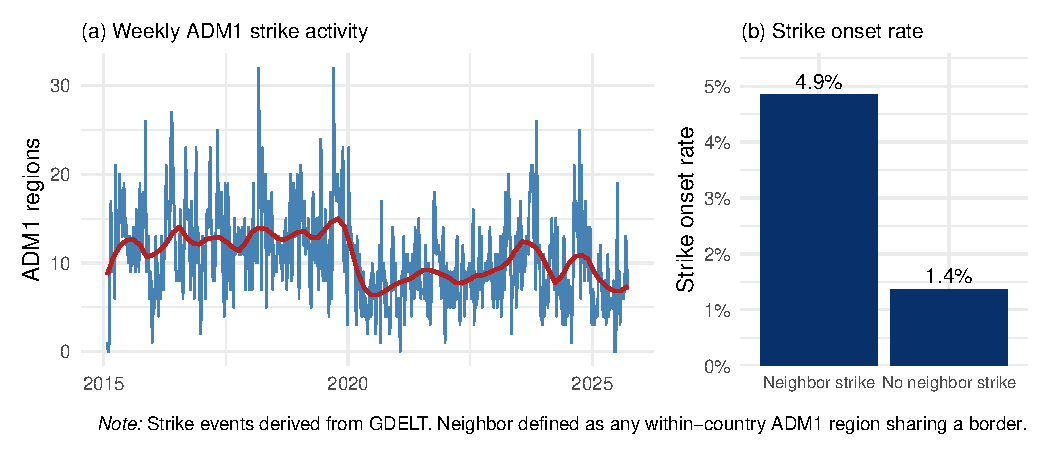
\includegraphics[keepaspectratio]{contagion-paper_files/figure-pdf/fig-puzzle-1.pdf}}

}

\caption{\label{fig-puzzle}Strike activity and neighbor exposure.}

\end{figure}%

\subsection{The National Foundations of Strike
Waves}\label{the-national-foundations-of-strike-waves}

The comparative-historical literature on strike waves consistently finds
that elevated strike activity sweeps multiple regions and industries
simultaneously rather than radiating outward from a geographic source.
Shorter and Tilly's (\citeproc{ref-shorter1974}{1974}) analysis of
French strike waves, Cronin's (\citeproc{ref-cronin1987}{1987})
documentation of the great British waves of 1871 to 1920, and Franzosi's
(\citeproc{ref-franzosi1989}{1989}, \citeproc{ref-franzosi1995}{1995})
analyses of Italian strikes all conclude that major waves are nationally
synchronized, driven by macro-level political and economic cycles that
create the same mobilization moment across regions at once. Strike waves
are synchronized in part because the relevant information, about
employer resistance and political opportunity, travels through national
media and union networks rather than through geographic proximity
(\citeproc{ref-biggs2002}{Biggs 2002}). Broad shifts in political
opportunity generate mobilization across sectors and regions
simultaneously, producing spatial clustering as a byproduct of common
national exposure rather than geographic spread
(\citeproc{ref-tarrow2011}{S. G. Tarrow 2011}).

Economic theories of strikes reinforce the primacy of national dynamics
from a different perspective. In the canonical bargaining model of
strikes, strike probability is a function of the gap between worker
expectations and firm capacity to pay, a gap driven by macroeconomic
conditions that are national in scope
(\citeproc{ref-ashenfelter1969}{Ashenfelter and Johnson 1969};
\citeproc{ref-kennan1993}{Kennan and Wilson 1993};
\citeproc{ref-card1990}{Card 1990}). When unexpected shifts in
profitability, inflation, or real wages affect all firms in a country
simultaneously, strike timing will be synchronized across regions not
because workers are imitating each other but because all face the same
economic environment. This synchronization has been documented
empirically at the macro level (\citeproc{ref-rees1952}{Rees 1952}) and
extended cross-nationally, with the late-1960s and early-1970s strike
waves across France, Italy, Britain, and the United States attributed to
shared macroeconomic and political conditions rather than sequential
contagion (\citeproc{ref-hibbs1976a}{Hibbs 1976},
\citeproc{ref-hibbs1978}{1978}).

\subsection{The Limits of Geographic
Contagion}\label{the-limits-of-geographic-contagion}

An established literature on the spatial diffusion of collective action
finds that geographic proximity predicts contagion, but largely for
violent and civil conflict rather than for labor organizing. Robust
neighborhood effects that survive structural controls have been
documented in studies of civil war onset
(\citeproc{ref-buhaug2008}{Buhaug and Gleditsch 2008}), with regional
conflict environments shaping civil war onset independently of domestic
conditions (\citeproc{ref-gleditsch2007}{Kristian Skrede Gleditsch
2007}). The mechanisms in these cases are local in character, including
rebel group expansion across borders, refugee flows that import
instability, ethnic networks spanning administrative boundaries, and
competition over natural resources that straddle frontiers.

None of these mechanisms translate straightforwardly to labor strikes.
The organizational infrastructure that translates mobilization signals
into strike action, including labor unions, collective bargaining
agreements, and labor law, operates overwhelmingly at the national level
(\citeproc{ref-shorter1974}{Shorter 1974};
\citeproc{ref-franzosi1995}{Franzosi 1995}). A union federation's
decision to call a general strike, or a government's announcement of
austerity measures, creates the same organizational moment for workers
in every region simultaneously. Geographic adjacency between
administrative units adds little to this national signal.

Even in the nonviolent protest literature, geographic neighbor effects
are weaker and more conditional than in conflict studies. The geographic
diffusion of nonviolent campaigns has been shown to depend on shared
political opportunity structures, with spatial proximity contributing
little once those structures are controlled
(\citeproc{ref-gleditsch2017}{Kristian S. Gleditsch and Rivera 2017}).
Genuine geographic diffusion requires active organizational brokerage,
with new ties deliberately constructed to link previously isolated
actors, and without such linkages what appears to be geographic spread
is better understood as simultaneous response to a common environment
(\citeproc{ref-tarrow2005}{S. Tarrow and McAdam 2005}).

\subsection{Institutional
Conditioning}\label{institutional-conditioning}

Even if national contagion predominates on average, the spatial
distribution of nationally-driven mobilization may vary with the
institutional context in which workers and employers operate. I consider
three dimensions of institutional context that may condition how strike
signals travel: freedom of expression, freedom of association, and state
repression.

Freedom of expression shapes the information infrastructure through
which national strike signals reach workers. Where press freedom is
strong and media access is broad, information about strikes travels
through national broadcast channels, reaching workers in all regions
simultaneously regardless of their geographic position. Collective
violence has been shown to diffuse along media distribution networks
rather than through geographic proximity (\citeproc{ref-myers2000}{Myers
2000}), and the same logic applies to strike news. Where national media
delivers the mobilization signal everywhere at once, no region needs a
striking neighbor to be activated, and the geographic structure of
strike waves should be correspondingly attenuated.

Freedom of association shapes the organizational infrastructure through
which workers translate national mobilization signals into local action.
Where associational rights are strong, dense union networks and civil
society organizations sustain direct linkages between workers, but those
networks are often locally embedded, organized at the plant, district,
or regional level rather than exclusively through national federations.
Where such locally structured networks are the primary conduit for
strike information and coordination (\citeproc{ref-biggs2002}{Biggs
2002}), geographic proximity becomes more rather than less important for
how the national signal propagates. Higher freedom of association should
therefore amplify the geographic structure of strike waves, producing
more spatially clustered national episodes.

State repression raises the costs of collective action and should
suppress the translation of strike signals into local mobilization.
Where states have the capacity and will to suppress collective action,
workers may observe strike activity nearby or perceive a national
mobilization wave and nonetheless not act, because the expected costs of
participation outweigh the informational update from the strike signal.
This logic has been demonstrated for conflict contagion
(\citeproc{ref-braithwaite2010}{Braithwaite 2010}), and the parallel
argument for strikes suggests that higher repression should dampen both
geographic and national transmission.

\subsection{Expectations}\label{expectations}

The arguments developed above yield five expectations, two concerning
the main contagion effects and three concerning institutional
conditioning. National contagion should be positive and substantial,
with the probability that any given region experiences strike activity
rising as a greater share of a country's regions are already mobilized,
reflecting the common national mobilization environment. Geographic
contagion, by contrast, should be negligible once national dynamics are
controlled, because spatial proximity between administrative units adds
little explanatory power beyond the national signal that is the primary
conduit for strike transmission.

The institutional conditioning arguments generate three further
expectations. Higher freedom of expression should attenuate the
geographic neighbor effect, as broadcast media substitutes for
geographic proximity as the primary conduit for strike signals. Higher
freedom of association should amplify it, as locally embedded
organizational networks reinforce the role of proximity in transmitting
mobilization. The opposite signs of these two predictions reflect a
single coherent theoretical claim: the two institutions route the same
national mobilization signal through different infrastructures, one that
flattens geographic structure and one that reinforces it. Higher
repression should dampen the translation of strike signals into local
mobilization through both channels.

\section{Data}\label{data}

\subsection{Strike Events: GDELT}\label{strike-events-gdelt}

The primary data source is the Global Database of Events, Language and
Tone (GDELT), a real-time database that codes news articles from global
media outlets into structured event records following the CAMEO coding
scheme (\citeproc{ref-leetaru2013a}{Leetaru and Schrodt 2013}). I
extract all events with CAMEO event codes beginning with ``143'' (labor
strikes and related actions) for the period January 2015 to September
2025, yielding approximately 30,900 events prior to filtering.

Each GDELT event record includes the action date, geographic coordinates
(\texttt{ActionGeo\_Lat}, \texttt{ActionGeo\_Long}), and a precision
indicator. I retain only events with valid coordinates and precision
codes indicating subnational geographic assignment. I spatially join
event coordinates to GADM version 4.1 administrative boundaries using
\texttt{sf::st\_join()} in R, assigning each event to its containing
ADM1 polygon. This coordinate-based matching achieves a 93\% assignment
rate.

\textbf{Coverage and bias.} GDELT's coverage is uneven across countries
and time. It relies on digitized English-language and multilingual news
sources, which generates systematic undercoverage in regions with
limited media presence, non-Latin scripts, or restricted press access.
The resulting panel therefore captures a selected subset of strike
activity, specifically events deemed newsworthy enough to receive media
coverage. This is a scope condition rather than a fatal flaw. The
analysis speaks to observable, newsworthy strikes rather than all strike
activity. Section 7 discusses the implications for interpretation.

\subsubsection{Panel Construction}\label{panel-construction}

I aggregate events to an ADM1-week panel spanning 2015--2025. The unit
of observation is an administrative region-week. The outcome variable is
a binary indicator for strike \emph{onset}, equal to one if at least one
strike event was recorded in the ADM1 unit during week \(t\), and zero
otherwise.\footnote{``Onset'' follows the epidemiological convention
  used in the conflict literature for first events within a defined
  window. In this context, it captures whether any new strike activity
  commenced in a region-week rather than whether activity was ongoing.
  The baseline onset rate across all ADM1-weeks is 1.4\%.}

The full panel includes {[}N{]} ADM1 units across {[}C{]} countries,
observed over {[}W{]} weeks, yielding {[}R{]} unit-week observations. I
exclude island ADM1 units with no contiguous within-country neighbors,
as they cannot receive geographic exposure and would contribute only
unexposed observations to the neighbor treatment variable.

\textbf{Figure 2} maps cumulative strike prevalence across ADM1 regions,
showing the number of weeks with recorded strike activity. Strike
activity is concentrated in South Asia, sub-Saharan Africa, and parts of
Europe, reflecting both true geographic variation and GDELT's media
coverage patterns.

\begin{figure}

\centering{

\pandocbounded{\includegraphics[keepaspectratio]{contagion-paper_files/figure-pdf/fig-data-1.pdf}}

}

\caption{\label{fig-data}Cumulative strike prevalence across ADM1
regions, 2015--2025.}

\end{figure}%

\subsection{Neighbor Relationships}\label{neighbor-relationships}

I define geographic neighbors as ADM1 units sharing a border within the
same country. I compute topological adjacency using
\texttt{spdep::poly2nb()} on GADM ADM1 polygons, separately identifying
within-country and cross-border adjacency. The main analysis uses
within-country neighbors. Cross-border adjacency is examined as an
exploratory extension.

\textbf{Table A1} (appendix) summarizes the distribution of neighbor
counts across ADM1 units.

\subsection{Treatment Variable}\label{treatment-variable}

The primary treatment variable is \texttt{neighbor\_strike\_t1\_t2}, a
binary indicator equal to one if at least one within-country geographic
neighbor had a strike onset in week \(t-1\) or week \(t-2\).

Neighbor strike exposure is rare. Only 7.9\% of ADM1-weeks have an
exposed neighbor. As shown in Figure 1b, however, exposure is strongly
associated with onset in the unconditional data. Exposed regions strike
at 4.9\% versus 1.4\% for unexposed regions, a 3.5-fold difference. The
empirical strategy addresses whether this raw association survives
conditioning on common shocks.

\subsection{National Contagion
Variable}\label{national-contagion-variable}

For the decomposition analysis (Section 5.2), I construct
\texttt{country\_share\_t1\_t2}, a normalized country-level exposure
measure equal to the proportion of other ADM1 regions in the same
country with a strike onset, averaged over weeks \(t-1\) and \(t-2\),
and normalized by \((N_c - 1)\) where \(N_c\) is the number of ADM1
units in country \(c\). This normalization ensures the measure is not
mechanically larger for countries with more administrative units.

\subsection{Institutional Moderators:
V-Dem}\label{institutional-moderators-v-dem}

I use three country-year indicators from the Varieties of Democracy
(V-Dem) project:

\begin{itemize}
\tightlist
\item
  \textbf{Freedom of expression} (\texttt{v2x\_freexp\_altinf}),
  measuring the extent of freedom of expression and media access
\item
  \textbf{Freedom of association} (\texttt{v2x\_frassoc\_thick}),
  measuring the extent of freedom of association and civil society
  participation
\item
  \textbf{State repression} (\texttt{v2x\_clphy}), measuring physical
  violence and intimidation by state agents
\end{itemize}

All three indicators are standardized (z-scored) before entering
interaction models, so the main treatment effect is interpreted at the
sample mean of each moderator.

\section{Empirical Strategy}\label{empirical-strategy}

The analysis tests the theoretical expectations through three
specifications. The first asks whether geographic neighbor exposure
predicts strike onset once national co-movement is absorbed, using a
two-way fixed effects design that pairs ADM1 unit fixed effects with
country-by-week fixed effects. The country-by-week fixed effects are the
key identifying restriction, absorbing all within-country variation in a
given week without requiring the researcher to specify which national
factors matter. A second specification estimates geographic and national
contagion simultaneously by replacing the country-by-week fixed effect
with an explicit measure of country-level strike activity, allowing both
effects to be compared directly in the same model. A third specification
then interacts the treatment variables with V-Dem indicators of freedom
of expression, freedom of association, and state repression to test
whether institutional context conditions the spatial structure of
diffusion.

\subsection{Two-Way Fixed Effects
Model}\label{two-way-fixed-effects-model}

To test whether geographic neighbor exposure predicts strike onset once
common national dynamics are removed, I estimate:

\[Y_{it} = \beta \cdot \text{NeighborStrike}_{i,t-1:t-2} + \alpha_i + \gamma_{c \times t} + \varepsilon_{it}\]

where \(Y_{it}\) is the binary strike onset indicator for ADM1 unit
\(i\) in week \(t\). The treatment variable
\(\text{NeighborStrike}_{i,t-1:t-2}\) is a binary indicator equal to one
if at least one within-country geographic neighbor recorded a strike
onset in week \(t-1\) or \(t-2\). I use two lags to capture a plausible
demonstration-effect window while keeping the treatment predetermined
with respect to the current period's outcome.

I estimate this as a linear probability model (LPM) via \texttt{feols}
in R (\citeproc{ref-berge2018}{Bergé 2018}). LPM is preferred over logit
in this setting because maximum likelihood estimators with many fixed
effects suffer from the incidental parameters problem, which does not
affect OLS (\citeproc{ref-lancaster2000}{Lancaster 2000};
\citeproc{ref-wooldridge2010}{Wooldridge 2010}). Coefficients are
directly interpretable as marginal effects on the probability of onset.
Given the low baseline onset rate of 1.4\%, I report a bias-corrected
logit robustness check using the \texttt{alpaca} package
(\citeproc{ref-fernandez-val2016}{\textbf{fernandez-val2016?}}) (see
Table A2). The substantive conclusions are unchanged.

Standard errors are clustered at the ADM1 level to account for serial
correlation within units over time. Ignoring within-unit serial
correlation in panel settings leads to substantially understated
standard errors (\citeproc{ref-bertrand2004}{Bertrand, Duflo, and
Mullainathan 2004}), and clustering at the ADM1 level is appropriate
because geographic neighbor exposure varies at that level
(\citeproc{ref-colincameron2015}{Colin Cameron and Miller 2015}).

The country-by-week fixed effect represents a more demanding
identification strategy than is typical in the conflict contagion
literature, which generally uses logit with parametric controls for
national conditions such as democracy, GDP per capita, and population
(\citeproc{ref-buhaug2008}{Buhaug and Gleditsch 2008};
\citeproc{ref-gleditsch2017}{Kristian S. Gleditsch and Rivera 2017}).
Rather than specifying which national factors to control for, the
saturated fixed effect absorbs all of them simultaneously. This approach
has been standard in the international trade literature, where
country-by-time fixed effects absorb unobservable common shocks without
requiring the researcher to model their form
(\citeproc{ref-baier2007}{Baier and Bergstrand 2007};
\citeproc{ref-head2014}{Head and Mayer 2014}). The lagged-treatment
design also has methodological precedent in the study of historical
collective action: Aidt, Leon, and Satchell
(\citeproc{ref-aidt2022a}{2022}) and Aidt and Leon
(\citeproc{ref-aidt2022}{2022}) employ a similar subnational spatial
panel approach to study the geographic diffusion of the English Swing
Riots of 1830--31. The present study extends this design to contemporary
global data and, unlike the Swing Riots case, finds no geographic
contagion once national dynamics are controlled. An alternative
framework would be an explicit spatial lag model, as in Arezki et al.
(\citeproc{ref-arezki2024}{2024}), who study protest contagion across
200 countries using a spatial autoregressive specification; however, the
lagged-treatment TWFE approach is preferred here because the
predetermined neighbor indicator avoids the simultaneity problem
inherent in contemporaneous spatial lags.

\subsection{National vs.~Geographic
Decomposition}\label{national-vs.-geographic-decomposition}

The central argument of the paper is that strike contagion operates at
the national rather than geographic level, and that the raw geographic
association in the data reflects common national dynamics rather than
direct transmission between neighboring regions. Testing this argument
requires estimating national and geographic contagion simultaneously. I
therefore replace the country-by-week fixed effect with an explicit
measure of country-level strike activity, constructing a specification
that places both channels in the same model:

\[Y_{it} = \beta_1 \cdot \text{NeighborStrike}_{i,t-1:t-2} + \beta_2 \cdot \text{CountryShare}_{i,t-1:t-2} + \alpha_i + \gamma_t + \varepsilon_{it}\]

where \(\gamma_t\) is a week fixed effect common to all countries and
\(\text{CountryShare}_{i,t-1:t-2}\) is the proportion of other ADM1
regions in the same country with a strike onset in \(t-1:t-2\),
normalized by \((N_c - 1)\) to remove any mechanical relationship with
country size. This specification estimates national contagion
(\(\beta_2\)) and the geographic neighbor effect net of national
activity (\(\beta_1\)) simultaneously. The parametric control is less
assumption-free than the saturated fixed effect but enables the
decomposition that the saturated approach forecloses. If the raw
geographic association reflects national rather than geographic
dynamics, as the theoretical framework predicts, \(\beta_2\) should be
large and positive while \(\beta_1\) collapses toward zero.

\subsection{Institutional Moderation}\label{institutional-moderation}

The third set of expectations concerns whether institutional context
conditions the spatial structure of diffusion. To test these, I interact
the neighbor strike treatment with V-Dem indicators:

\[Y_{it} = \beta_1 \cdot \text{NeighborStrike}_{it} + \beta_2 \cdot \text{Institution}_{ct} + \beta_3 \cdot (\text{NeighborStrike}_{it} \times \text{Institution}_{ct}) + \alpha_i + \gamma_t + \varepsilon_{it}\]

These specifications draw on cross-national variation in institutional
context to test whether the structure of diffusion varies with the
political environment in which workers operate. I use ADM1 and week
fixed effects with \(\text{CountryShare}\) as a control for national
waves, identifying the moderation effects primarily from between-country
differences in institutional context. The estimates are therefore best
read as descriptive of cross-national heterogeneity rather than
within-country causal moderation. All V-Dem indicators are standardized
so that the main treatment coefficient is interpreted at the sample mean
of each moderator.

\section{Results}\label{results}

The analysis proceeds in three stages. First, I estimate the baseline
effect of geographic neighbor strike exposure using a two-way fixed
effects strategy that absorbs common national shocks. Second, I
decompose the apparent neighborhood effect into national and geographic
channels. Third, I examine whether institutional context conditions the
geographic structure of strike contagion.

\subsection{Geographic Neighbor
Exposure}\label{geographic-neighbor-exposure}

Table 1 presents baseline results from the ADM1 and country-by-week
fixed effects model. Geographic neighbor strike exposure does not
significantly predict strike onset once common within-country shocks are
absorbed, a striking result given the raw association (see Figure 1).
Country-by-week fixed effects fully absorb this association, indicating
the raw correlation reflects common national dynamics rather than
geographic diffusion.

\begingroup
\centering
\begin{table}
\caption{Baseline specification: neighbor strike exposure and strike onset}\tabularnewline

\centering
\begin{tabular}{lccc}
   \hline
    & \multicolumn{3}{c}{strike\_onset}\\
   Model:                         & (i)      & (ii)           & (iii)\\  
   \midrule
   \emph{Variables}\\
   Neighbor strike (t$-$1, t$-$2) & -0.0031  &                &   \\   
                                  & (0.0021) &                &   \\   
   Neighbor strike (t$-$1 only)   &          & -0.0058$^{**}$ &   \\   
                                  &          & (0.0027)       &   \\   
   Neighbor strike (t$-$2 only)   &          &                & -0.0014\\   
                                  &          &                & (0.0023)\\   
   \midrule
   \emph{Fixed-effects}\\
   ADM1                           & Yes      & Yes            & Yes\\  
   Country $\times$ Week          & Yes      & Yes            & Yes\\  
   \midrule
   \emph{Fit statistics}\\
   Observations                   & 315,808  & 315,808        & 315,240\\  
   R$^2$                          & 0.19665  & 0.19668        & 0.19670\\  
   \hline
   \multicolumn{4}{l}{\emph{Clustered (ADM1) standard-errors in parentheses}}\\
   \multicolumn{4}{l}{\emph{Signif. Codes: ***: 0.01, **: 0.05, *: 0.1}}\\
\end{tabular}
\end{table}

\par\endgroup

Examining the two lags separately sharpens the picture. The t−1 lag is
negative and marginally significant (β = −0.006, p = 0.036), while the
t−2 lag is null. Rather than pointing to a modest diffusion effect at
one lag, the negative t−1 coefficient suggests a displacement or
substitution dynamic in which the focal region becomes \emph{less}
likely to follow immediately once a neighboring region strikes, a
pattern discussed further below.

\subsection{National vs.~Neighborhood
Decomposition}\label{national-vs.-neighborhood-decomposition}

Table 2 decomposes geographic and national contagion by replacing the
country-by-week fixed effect with the country strike share measure
alongside the geographic neighbor indicator. Column (1) establishes that
national-level contagion is large and highly significant. A one
percentage-point increase in the country strike share raises the focal
region's onset probability by 0.66 percentage points, a near-doubling of
onset risk at a one-standard-deviation increase, and national contagion
alone explains 6.3\% of within-unit variance, a substantial share given
the sparseness of the outcome.

\begingroup
\centering
\begin{table}
\caption{National vs.~neighborhood decomposition}\tabularnewline

\centering
\begin{tabular}{lccc}
   \hline
    & \multicolumn{3}{c}{strike\_onset}\\
   Model:                         & (i)            & (ii)           & (iii)\\  
   \midrule
   \emph{Variables}\\
   Country share (t$-$1, t$-$2)   & 0.6620$^{***}$ &                & 0.6653$^{***}$\\   
                                  & (0.0501)       &                & (0.0507)\\   
   Neighbor strike (t$-$1, t$-$2) &                & 0.0149$^{***}$ & -0.0043$^{**}$\\   
                                  &                & (0.0018)       & (0.0020)\\   
   \midrule
   \emph{Fixed-effects}\\
   ADM1                           & Yes            & Yes            & Yes\\  
   Week                           & Yes            & Yes            & Yes\\  
   \midrule
   \emph{Fit statistics}\\
   Observations                   & 315,808        & 315,808        & 315,808\\  
   R$^2$                          & 0.13925        & 0.08181        & 0.13931\\  
   \hline
   \multicolumn{4}{l}{\emph{Clustered (ADM1) standard-errors in parentheses}}\\
   \multicolumn{4}{l}{\emph{Signif. Codes: ***: 0.01, **: 0.05, *: 0.1}}\\
\end{tabular}
\end{table}

\par\endgroup

Column (2) isolates the geographic neighbor effect. In the absence of
controls for national activity, having a striking neighbor is positive
and significant (+1.5 percentage points, p \textless{} 0.001),
consistent with prior literature on geographic diffusion.

However, column (3) is the key specification. When both measures are
included simultaneously, the national share coefficient is unchanged
(+0.665, p \textless{} 0.001) while the geographic neighbor effect
reverses sign (β = −0.004, p = 0.035). Once national activity is
controlled, having a geographically adjacent neighbor strike slightly
reduces the focal region's onset probability.

The contrast in explanatory power is stark. National contagion explains
63 times more within-unit variance than geographic neighbor exposure
(within R² = 0.063 versus 0.001). The 1.5 percentage-point neighborhood
effect in column (2) is entirely attributable to national wave dynamics.
Workers in the same country tend to strike together not because
geographic proximity transmits the mobilization signal, but because a
common national dynamic drives coordinated action.\footnote{The negative
  coefficient on the geographic neighbor indicator should be interpreted
  with caution. It is identified from the narrow set of cases where a
  region's neighbors diverge from national trends, a relatively rare
  occurrence by construction, and is therefore estimated from thinner
  variation than the country share coefficient.}

\subsection{Institutional Moderation}\label{institutional-moderation-1}

Table 3 examines whether institutional context conditions the geographic
structure of strike waves. I interact the neighbor strike treatment and
the country share measure with three V-Dem indicators (freedom of
expression, freedom of association, and state repression), entered
individually and jointly, using ADM1 and week fixed effects with country
share as a parametric control for national waves.

\begingroup
\centering
\begin{table}
\caption{Institutional moderation of geographic and national contagion}\tabularnewline

\centering
\begin{tabular}{lcccc}
   \hline
    & \multicolumn{4}{c}{strike\_onset}\\
   Model:                                & (i)            & (ii)            & (iii)          & (iv)\\  
   \midrule
   \emph{Variables}\\
   Neighbor strike (t$-$1, t$-$2)        & -0.0047$^{**}$ & -0.0060$^{***}$ & -0.0046$^{**}$ & -0.0067$^{***}$\\   
                                         & (0.0021)       & (0.0020)        & (0.0020)       & (0.0020)\\   
   Freedom of expression (z)             & 0.0001         &                 &                & 0.0004\\   
                                         & (0.0015)       &                 &                & (0.0029)\\   
   Country share (t$-$1, t$-$2)          & 0.6544$^{***}$ & 0.6507$^{***}$  & 0.6588$^{***}$ & 0.6507$^{***}$\\   
                                         & (0.0496)       & (0.0489)        & (0.0496)       & (0.0493)\\   
   Neighbor strike $\times$ Expression   & 0.0018         &                 &                & -0.0121$^{**}$\\   
                                         & (0.0022)       &                 &                & (0.0054)\\   
   Country share $\times$ Expression     & 0.0551         &                 &                & 0.0561\\   
                                         & (0.0469)       &                 &                & (0.1535)\\   
   Freedom of association (z)            &                & -0.0004         &                & -0.0016\\   
                                         &                & (0.0019)        &                & (0.0028)\\   
   Neighbor strike $\times$ Association  &                & 0.0045$^{**}$   &                & 0.0157$^{***}$\\   
                                         &                & (0.0023)        &                & (0.0058)\\   
   Country share $\times$ Association    &                & 0.0618          &                & 0.0542\\   
                                         &                & (0.0477)        &                & (0.1351)\\   
   State repression (z)                  &                &                 & 0.0005         & 0.0012\\   
                                         &                &                 & (0.0013)       & (0.0020)\\   
   Neighbor strike $\times$ Repression   &                &                 & 0.0024         & 0.0010\\   
                                         &                &                 & (0.0021)       & (0.0024)\\   
   Country share $\times$ Repression     &                &                 & 0.0295         & -0.0507\\   
                                         &                &                 & (0.0451)       & (0.0774)\\   
   \midrule
   \emph{Fixed-effects}\\
   ADM1                                  & Yes            & Yes             & Yes            & Yes\\  
   Week                                  & Yes            & Yes             & Yes            & Yes\\  
   \midrule
   \emph{Fit statistics}\\
   Observations                          & 294,224        & 294,224         & 294,224        & 294,224\\  
   R$^2$                                 & 0.14130        & 0.14136         & 0.14109        & 0.14151\\  
   \hline
   \multicolumn{5}{l}{\emph{Clustered (ADM1) standard-errors in parentheses}}\\
   \multicolumn{5}{l}{\emph{Signif. Codes: ***: 0.01, **: 0.05, *: 0.1}}\\
\end{tabular}
\end{table}

\par\endgroup

Institutional context does not condition how strongly national strike
waves propagate. The country share interactions are null across all
three moderators and in the joint model, and any conditioning operates
exclusively on the geographic channel. When modeled jointly, freedom of
expression attenuates the neighbor strike effect (β = −0.009, p = 0.073)
while freedom of association amplifies it (β = +0.010, p = 0.062), with
effects that are nearly equal in magnitude and opposite in sign.
Repression is null throughout. When modeled separately, these effects
are attenuated because freedom of expression and freedom of association
are positively correlated and their opposing effects partially cancel
when either is included in isolation.

In countries with strong freedom of expression, information about
strikes spreads rapidly through national media, enabling workers in
distant regions to coordinate simultaneously rather than through
geographic proximity, producing nationally homogeneous strike waves with
little geographic gradient. In countries with strong freedom of
association, dense union networks are locally embedded at the plant,
district, or regional level, creating organizational infrastructure that
reinforces the role of geographic proximity in transmitting mobilization
signals, producing geographically structured national episodes rather
than uniform waves. In short, freedom of expression produces nationally
homogeneous strike waves while freedom of association produces
geographically structured ones.

These results must be qualified by the decomposition finding. Since the
geographic neighbor effect approaches zero and turns negative once
country-level contagion is controlled, the moderation results are best
understood as capturing the spatial structure of nationally-driven
mobilization rather than true neighborhood diffusion. Institutions shape
how national strike waves distribute across space but do not appear to
generate or amplify geographic transmission as an independent mechanism.

\subsection{Robustness}\label{robustness}

The null geographic contagion result is robust across alternative
specifications. Two-way clustering and logistic regression leave the
main findings unchanged (Table A2). Results also replicate in the
validated-location subsample, which restricts to strike events with
confirmed ADM1 geocodes (Tables A3 and A4), with the null geographic
neighbor effect and large national contagion both intact. Cross-border
neighbor exposure is null across all specifications (Table A5),
consistent with the view that strike contagion is bounded by national
institutional frameworks.

\section{Discussion}\label{discussion}

The results establish three robust findings: geographic neighbor
exposure has no independent effect on strike onset once national
dynamics are controlled; national contagion is large and explains orders
of magnitude more within-unit variance than geographic proximity; and
civil liberties shape the spatial structure of nationally-driven
mobilization without conditioning its overall strength. Together these
findings suggest that future research should focus on understanding what
produces national synchronization and how institutions determine whether
that synchronization takes a geographically uniform or spatially
clustered form. This discussion highlights three questions related to
this task. What drives national strike waves and what would it take to
study them? Why do institutional conditioning effects appear modest and
difficult to pin down? And does the contagion process look different for
different types of strikes?

\subsection{Why Institutional Conditioning Is Hard to Pin
Down}\label{why-institutional-conditioning-is-hard-to-pin-down}

While the institutional moderation results are theoretically coherent,
the estimates are limited by two key factors. The first is a fundamental
measurement issue. GDELT's media-derived event detection is
systematically thinner in high-repression environments. In countries
where the state actively restricts press access, suppresses protest
reporting, or controls media outlets, the observable strike record is
likely a highly selected sample of actual labor activity, capturing only
the most egregious, internationally newsworthy episodes rather than the
full distribution of strike behavior that the theory targets. Repression
both suppresses the mobilization the analysis is trying to detect and
degrades the measurement instrument simultaneously. As a result, a null
result in this context cannot be interpreted as a genuine null.

A second problem affects all three V-Dem moderators. Freedom of
expression, freedom of association, and state repression are measured
annually at the country level and move very slowly over time. As a
result, identifying variation in the interaction terms is almost
entirely cross-sectional and indicates whether countries with higher
civil liberties show different geographic strike structures as opposed
to whether a country's strike geography changes as its institutions
evolve. ADM1 and week fixed effects cannot absorb the many ways that
high-civil-liberty countries differ from low-civil-liberty countries,
including levels of development, state capacity, democratic
consolidation, and union density, so the moderation estimates should be
interpreted as exploratory cross-national comparisons rather than causal
estimates of institutional effects.

Resolving these problems requires measures with substantially more
temporal variation. One promising direction draws on the same event-data
infrastructure used to construct the strike panel itself. GDELT's Global
Knowledge Graph codes thematic content of news articles including media
censorship events, and actor-type codes identify labor organizations,
civil society groups, and government coercion events. From these it is
possible, in principle, to construct country-month or even country-week
proxies for information environment (volume and source diversity of
media coverage, frequency of censorship-related events) and
associational density (frequency of labor organization and civil society
mentions). ACLED provides event-level data on state violence against
protesters at weekly resolution across more than 150 countries, which
could serve as a dynamic repression measure that varies within country
over time. The advantage of these alternatives is precisely that they
would generate within-country temporal variation, allowing the
moderation analysis to be identified from changes in institutional
context within a country rather than from cross-country comparisons, and
making it possible to absorb country-level unobservables in a way that
the current approach cannot.

Freedom of expression and freedom of association are also positively
correlated across countries, which limits the ability to identify their
opposing effects when either enters the model in isolation. This is why
the joint model is the appropriate specification, but even there the
estimates are noisier than they would be if the two institutions were
orthogonal. Direct measures of the underlying mechanisms, including
media reach across subnational regions, local union density at the ADM1
level, or other measures of associational infrastructure, could provide
sharper tests of the theoretical claims than annual national indices
that bundle many distinct institutional features into a single score.

\subsection{What Drives National Strike
Waves?}\label{what-drives-national-strike-waves}

The two-way fixed effects design is conservative by construction:
country-by-week fixed effects absorb all national common shocks,
including the wave dynamics that the large national contagion effect
implies are present and substantial. This conservatism is the right
choice for the geographic contagion test, but it purchases
identification at the cost of any information about what generates
national waves in the first place. The current paper establishes that
when national waves occur they produce large and spatially broad
increases in strike probability, but what triggers them remains
unexamined.

A natural extension of this research is a country-week or
country-quarter model of aggregate strike activity, asking what economic
and political conditions predict entry into high-strike periods. The
macroeconomic drivers of strike waves are well-theorized. Wage-price
cycles, unexpected shifts in firm profitability, unemployment
trajectories, and real wage growth have all been implicated in the
historical wave literature, and these can be approximated from IMF and
World Bank sources at quarterly frequency. The political opportunity
literature points to government partisanship, election cycles, and
austerity episodes as triggers for politically timed waves; here V-Dem
and ParlGov provide the relevant variables. Union density and bargaining
centralization from the OECD and ILO would capture the organizational
infrastructure that converts economic grievances into coordinated action
for at least a subset of countries. Contract cycle dynamics, whereby
periods when many workers' agreements come up for renewal simultaneously
create windows of elevated strike risk, could also be examined using ILO
labor statistics where available, and GDELT-derived time series of labor
negotiation events and wage-related news coverage could serve as leading
indicators in countries where official statistics are sparse.

\subsection{Strike Types and the Geography of
Mobilization}\label{strike-types-and-the-geography-of-mobilization}

A third question concerns whether the contagion process looks the same
across different types of strikes. The current analysis treats all CAMEO
143 events as equivalent, aggregating general strikes, industrial
strikes, and political protest strikes into a single onset indicator.
This may obscure substantial heterogeneity in how different kinds of
labor action spread, and may explain at least part of why geographic and
national channels behave as they do in the aggregate.

The contrast between industry-specific and general strikes is
theoretically sharp. Workers in particular industries are often
geographically concentrated. Coal mines cluster in mining regions,
garment factories in export processing zones, port workers in coastal
cities, while public school teachers are distributed across every
administrative region simultaneously. A wage dispute in a textile
corridor may produce correlated strike activity in neighboring textile
regions through genuine industry-network channels, including shared
union federations, the same employer association, and synchronized
contract cycles, while having no effect on non-textile regions in the
same country. This pattern would look like geographic contagion in the
raw data and would survive some national controls, even though the
mechanism is sectoral rather than spatial. The current design cannot
rule out that spatially clustered sectors account for the modest
geographic residuals identified here. Disaggregating by industry would
make this testable directly.

General strikes, by contrast, are inherently national by their
organizational logic. They are typically called by national labor
federations or peak union bodies in response to national policy
decisions such as austerity packages, labor law reform, pension cuts, or
anti-privatization campaigns, and are designed to achieve simultaneous
participation across all sectors and regions. The geographic structure
of general strikes should therefore be strongly nationally homogeneous,
not because spatial transmission fails but because the organizing logic
is explicitly national. Political strikes targeting the government
rather than a specific employer follow a similar logic and should
similarly display national rather than geographic structure.

Public-sector and private-sector strikes represent a related dimension.
Public-sector workers in many countries face a single national employer,
are subject to nationally-set wage scales and budget cycles, and are
organized through federations that negotiate at the national level. A
government announcement of public-sector pay restraint creates the same
mobilization moment simultaneously across states and provinces in a way
that a private-sector wage dispute in one factory does not.
Private-sector strikes, where wages are negotiated at the plant or
sector level, should show more spatial heterogeneity.

Testing these distinctions is within reach using the existing LLM
classification infrastructure. The URL and headline classification
pipeline developed for event validation, which already identifies
whether a GDELT event represents a genuine strike, can be extended to
classify strike type using the same few-shot prompting approach applied
to the same underlying article text and metadata. Classifying events as
general or sectoral, public- or private-sector, industrial or political
requires additional annotation effort and prompt engineering but no new
architectural decisions. Industry classification from article text,
covering sectors such as mining, transport, education, healthcare, and
manufacturing, would permit a more granular decomposition.

\section{Conclusion}\label{conclusion}

This paper set out to ask whether strikes spread geographically, whether
seeing a neighbor strike makes you more likely to strike. The answer, at
least at the subnational level with weekly data from 181 countries, is
no. The spatial clustering of strikes is real, but it reflects the
national structure of strike waves. When a country is in a period of
labor mobilization, all its regions tend to strike together. Geography
per se does not amplify or structure this transmission.

The positive finding --- large, robust national contagion effects ---
opens an agenda for understanding what drives national strike waves. Why
do some countries experience synchronized national waves while others
see more localized episodes? What roles do national union federations,
political cycles, and macroeconomic shocks play in generating and
sustaining national waves? These questions are not answerable with the
current design, which absorbs national wave dynamics into fixed effects,
but they suggest productive directions for future research.

\newpage

\section{References}\label{references}

\setlength{\parindent}{-0.2in}
\setlength{\leftskip}{0.2in}
\setlength{\parskip}{8pt}
\noindent

\phantomsection\label{refs}
\begin{CSLReferences}{1}{0}
\bibitem[\citeproctext]{ref-aidt2022}
Aidt, Toke, and Gabriel Leon-Ablan. 2022. {``The {Interaction} of
{Structural Factors} and {Diffusion} in {Social Unrest}: {Evidence} from
the {Swing Riots}.''} \emph{British Journal of Political Science} 52
(2): 869--85. \url{https://doi.org/10.1017/S0007123420000873}.

\bibitem[\citeproctext]{ref-aidt2022a}
Aidt, Toke, Gabriel Leon-Ablan, and Max Satchell. 2022. {``The {Social
Dynamics} of {Collective Action}: {Evidence} from the {Diffusion} of the
{Swing Riots}, 1830--1831.''} \emph{The Journal of Politics} 84 (1):
209--25. \url{https://doi.org/10.1086/714784}.

\bibitem[\citeproctext]{ref-arezki2024}
Arezki, Rabah, Alou Adesse Dama, Simeon Djankov, and Ha Nguyen. 2024.
{``Contagious Protests.''} \emph{Empirical Economics} 66 (6):
2397--2434. \url{https://doi.org/10.1007/s00181-023-02539-y}.

\bibitem[\citeproctext]{ref-ashenfelter1969}
Ashenfelter, Orley, and George E. Johnson. 1969. {``Bargaining {Theory},
{Trade Unions}, and {Industrial Strike Activity}.''} \emph{The American
Economic Review} 59 (1): 35--49.
\url{http://www.jstor.org/stable/1811091}.

\bibitem[\citeproctext]{ref-baier2007}
Baier, Scott L., and Jeffrey H. Bergstrand. 2007. {``Do Free Trade
Agreements Actually Increase Members' International Trade?''}
\emph{Journal of International Economics} 71 (1): 72--95.
\url{https://doi.org/10.1016/j.jinteco.2006.02.005}.

\bibitem[\citeproctext]{ref-berge2018}
Bergé, Laurent. 2018. {``Efficient Estimation of Maximum Likelihood
Models with Multiple Fixed-Effects: The {R} Package {FENmlm}.''} Working
paper. Department of Economics at the University of Luxembourg.
\url{https://EconPapers.repec.org/RePEc:luc:wpaper:18-13}.

\bibitem[\citeproctext]{ref-bertrand2004}
Bertrand, M., E. Duflo, and S. Mullainathan. 2004. {``How {Much Should
We Trust Differences-In-Differences Estimates}?''} \emph{The Quarterly
Journal of Economics} 119 (1): 249--75.
\url{https://doi.org/10.1162/003355304772839588}.

\bibitem[\citeproctext]{ref-biggs2002}
Biggs, Michael. 2002. {``Strikes as {Sequences} of {Interaction}: {The
American Strike Wave} of 1886.''} \emph{Social Science History} 26 (3):
583--617. \url{https://doi.org/10.1017/S0145553200013092}.

\bibitem[\citeproctext]{ref-braithwaite2010}
Braithwaite, Alex. 2010. {``Resisting Infection: {How} State Capacity
Conditions Conflict Contagion.''} \emph{Journal of Peace Research} 47
(3): 311--19. \url{https://doi.org/10.1177/0022343310362164}.

\bibitem[\citeproctext]{ref-buhaug2008}
Buhaug, Halvard, and Kristian Skrede Gleditsch. 2008. {``Contagion or
{Confusion}? {Why Conflicts Cluster} in {Space}.''} \emph{International
Studies Quarterly} 52 (2): 215--33.
\url{https://doi.org/10.1111/j.1468-2478.2008.00499.x}.

\bibitem[\citeproctext]{ref-card1990}
Card, David. 1990. {``Strikes and {Wages}: {A Test} of an {Asymmetric
Information Model}.''} \emph{The Quarterly Journal of Economics} 105
(3): 625. \url{https://doi.org/10.2307/2937893}.

\bibitem[\citeproctext]{ref-colincameron2015}
Colin Cameron, A., and Douglas L. Miller. 2015. {``A {Practitioner}'s
{Guide} to {Cluster-Robust Inference}.''} \emph{Journal of Human
Resources} 50 (2): 317--72. \url{https://doi.org/10.3368/jhr.50.2.317}.

\bibitem[\citeproctext]{ref-cronin1987}
Cronin, James E. 1987. {``Strikes and {Power} in {Britain},
1870-1920.''} \emph{International Review of Social History} 32 (2):
144--67. \url{https://www.jstor.org/stable/44581972}.

\bibitem[\citeproctext]{ref-franzosi1989}
Franzosi, Roberto. 1989. {``One {Hundred Years} of {Strike Statistics}:
{Methodological} and {Theoretical Issues} in {Quantitative Strike
Research}.''} \emph{ILR Review} 42 (3): 348--62.
\url{https://doi.org/10.1177/001979398904200302}.

\bibitem[\citeproctext]{ref-franzosi1995}
---------. 1995. \emph{The {Puzzle} of {Strikes}: {Class} and {State
Strategies} in {Postwar Italy}}. 1st ed. Cambridge University Press.
\url{https://doi.org/10.1017/CBO9780511571534}.

\bibitem[\citeproctext]{ref-gleditsch2007}
Gleditsch, Kristian Skrede. 2007. {``Transnational {Dimensions} of
{Civil War}.''} \emph{Journal of Peace Research} 44 (3): 293--309.
\url{https://doi.org/10.1177/0022343307076637}.

\bibitem[\citeproctext]{ref-gleditsch2017}
Gleditsch, Kristian S., and Mauricio Rivera. 2017. {``The {Diffusion} of
{Nonviolent Campaigns}.''} \emph{Journal of Conflict Resolution} 61 (5):
1120--45. \url{https://doi.org/10.1177/0022002715603101}.

\bibitem[\citeproctext]{ref-granovetter1978}
Granovetter, Mark. 1978. {``Threshold {Models} of {Collective
Behavior}.''} \emph{American Journal of Sociology} 83 (6): 1420--43.
\url{https://doi.org/10.1086/226707}.

\bibitem[\citeproctext]{ref-head2014}
Head, Keith, and Thierry Mayer. 2014. {``Gravity {Equations}:
{Workhorse},{Toolkit}, and {Cookbook}.''} In \emph{Handbook of
{International Economics}}, 4:131--95. Elsevier.
\url{https://doi.org/10.1016/B978-0-444-54314-1.00003-3}.

\bibitem[\citeproctext]{ref-hibbs1976a}
Hibbs, Douglas A. 1976. {``Industrial {Conflict} in {Advanced Industrial
Societies}.''} \emph{American Political Science Review} 70 (4):
1033--58. \url{https://doi.org/10.2307/1959373}.

\bibitem[\citeproctext]{ref-hibbs1978}
---------. 1978. {``On the {Political Economy} of {Long-Run Trends} in
{Strike Activity}.''} \emph{British Journal of Political Science} 8 (2):
153--75. \url{https://doi.org/10.1017/S0007123400001289}.

\bibitem[\citeproctext]{ref-kennan1993}
Kennan, John, and Robert Wilson. 1993. {``Bargaining with Private
Information.''} \emph{Journal of Economic Literature} 31 (1): 45--104.
\url{http://www.jstor.org/stable/2728150}.

\bibitem[\citeproctext]{ref-lancaster2000}
Lancaster, Tony. 2000. {``The Incidental Parameter Problem Since
1948.''} \emph{Journal of Econometrics} 95 (2): 391--413.
\url{https://doi.org/10.1016/S0304-4076(99)00044-5}.

\bibitem[\citeproctext]{ref-leetaru2013a}
Leetaru, Kalev, and Philip A Schrodt. 2013. {``{GDELT}: {Global Data} on
{Events}, {Location} and {Tone},''}

\bibitem[\citeproctext]{ref-mcadam2008}
McAdam, Doug, Sidney G. Tarrow, Charles Tilly, and Sidney G. Tarrow.
2008. \emph{Dynamics of Contention}. Reprinted. Cambridge Studies in
Contentious Politics. Cambridge: Cambridge University Press.

\bibitem[\citeproctext]{ref-myers2000}
Myers, Daniel J. 2000. {``The {Diffusion} of {Collective Violence}:
{Infectiousness}, {Susceptibility}, and {Mass Media Networks}.''}
\emph{American Journal of Sociology} 106 (1): 173--208.
\url{https://doi.org/10.1086/303110}.

\bibitem[\citeproctext]{ref-oliver2003}
Oliver, Pamela E., and Daniel J. Myers. 2003. {``Networks, {Diffusion},
and {Cycles} of {Collective Action}.''} In \emph{Social {Movements} and
{Networks}}, edited by Mario Diani and Doug McAdam, 1st ed., 173--203.
Oxford University PressOxford.
\url{https://doi.org/10.1093/0199251789.003.0008}.

\bibitem[\citeproctext]{ref-rees1952}
Rees, Albert. 1952. {``Industrial {Conflict} and {Business
Fluctuations}.''} \emph{Journal of Political Economy} 60 (5): 371--82.
\url{https://www.jstor.org/stable/1826482}.

\bibitem[\citeproctext]{ref-shorter1974}
Shorter, Edward. 1974. \emph{Strikes in {France}, 1830-1968}. London:
Cambridge University Press.

\bibitem[\citeproctext]{ref-tarrow2011}
Tarrow, Sidney G. 2011. \emph{Power in Movement: Social Movements and
Contentious Politics}. Rev. \& updated 3rd ed (Online-Ausg.). Cambridge
{Studies} in {Comparative Politics}. Cambridge New York: Cambridge
University Press.

\bibitem[\citeproctext]{ref-tarrow2005}
Tarrow, Sidney, and Doug McAdam. 2005. {``Scale Shift in Transnational
Contention.''} \emph{Transnational Protest and Global Activism} 121:
146.

\bibitem[\citeproctext]{ref-wooldridge2010}
Wooldridge, Jeffrey M. 2010. \emph{Econometric Analysis of Cross Section
and Panel Data}. 2nd ed. Cambridge, Mass: MIT Press.

\end{CSLReferences}

\clearpage
\FloatBarrier
\appendix
\renewcommand{\thetable}{A\arabic{table}}
\renewcommand{\thefigure}{A\arabic{figure}}
\setcounter{table}{0}
\setcounter{figure}{0}
\setlength{\parindent}{0.5in}
\setlength{\leftskip}{0in}
\setlength{\parskip}{0em}

\section{Appendix}\label{appendix}

\subsection{Summary Statistics}\label{summary-statistics}

\begin{longtable}[]{@{}llllll@{}}

\caption{\label{tbl-sumstats}Summary statistics for the analysis sample}

\tabularnewline

\toprule\noalign{}
& N & Mean & SD & Min & Max \\
\midrule\noalign{}
\endhead
\bottomrule\noalign{}
\endlastfoot
Strike onset & 315808 & 0.016 & 0.127 & 0.000 & 1.000 \\
Neighbor strike (t-1, t-2) & 315808 & 0.079 & 0.269 & 0.000 & 1.000 \\
Freedom of expression (z) & 294224 & 0.012 & 1.006 & -2.434 & 1.013 \\
Freedom of association (z) & 294224 & 0.018 & 0.998 & -2.537 & 0.928 \\
State repression (z) & 294224 & -0.042 & 0.998 & -2.372 & 1.103 \\

\end{longtable}

\subsection{Alternative
Specifications}\label{alternative-specifications}

\textbf{Table A2} replicates the baseline under two alternative
specifications: two-way clustering of standard errors at both the ADM1
and country-week levels, and logistic regression. Results are
qualitatively identical across all three. The null geographic neighbor
effect is not an artifact of the standard error choice or the linear
probability model.

\begingroup
\centering
\begin{table}
\caption{Robustness: alternative standard errors and estimator}\tabularnewline

\centering
\begin{tabular}{lccc}
   \hline
    & \multicolumn{3}{c}{strike\_onset}\\
   Model:                         & (i)      & (ii)     & (iii)\\  
                                  &  OLS     & OLS      & Logit\\  
   \midrule
   \emph{Variables}\\
   Neighbor strike (t$-$1, t$-$2) & -0.0031  & -0.0031  & -0.0576\\   
                                  & (0.0021) & (0.0020) & (0.0660)\\   
   \midrule
   \emph{Fixed-effects}\\
   ADM1                           & Yes      & Yes      & Yes\\  
   Country $\times$ Week          & Yes      & Yes      & Yes\\  
   \midrule
   \emph{Fit statistics}\\
   Observations                   & 315,808  & 315,808  & 58,839\\  
   R$^2$                          & 0.19665  & 0.19665  & \\  
   \hline
   \multicolumn{4}{l}{\emph{Signif. Codes: ***: 0.01, **: 0.05, *: 0.1}}\\
\end{tabular}
\end{table}

\par\endgroup

\subsection{Validated-Location
Robustness}\label{validated-location-robustness}

The following tables replicate the main results restricting to strike
events where the ADM1 geocode was confirmed correct by the LLM-based
geo-validation step (\texttt{geo\_quality\ ==\ "validated"}).
Unvalidated strike weeks are recoded as non-onset weeks, keeping the
balanced panel intact. The validated sample has an onset rate of
approximately 0.87\% compared to 1.4\% in the full sample. \textbf{Table
A3} compares the baseline model across samples. \textbf{Table A4}
compares the decomposition.

\begingroup
\centering
\begin{table}
\caption{Validated-location robustness: baseline specification}\tabularnewline

\centering
\begin{tabular}{lcc}
   \hline
                                  & strike\_onset  & strike\_onset\_val\\    
   Model:                         & (i)            & (ii)\\  
   \midrule
   \emph{Variables}\\
   Neighbor strike (t$-$1, t$-$2) & -0.0031        & -0.0017\\   
                                  & (0.0021)       & (0.0015)\\   
   \midrule
   \emph{Fixed-effects}\\
   ADM1                           & Yes            & Yes\\  
   Country $\times$ Week          & Yes            & Yes\\  
   \midrule
   \emph{Fit statistics}\\
   Observations                   & 315,808        & 315,808\\  
   R$^2$                          & 0.19665        & 0.14678\\  
   \hline
   \multicolumn{3}{l}{\emph{Clustered (ADM1) standard-errors in parentheses}}\\
   \multicolumn{3}{l}{\emph{Signif. Codes: ***: 0.01, **: 0.05, *: 0.1}}\\
\end{tabular}
\end{table}

\par\endgroup

\begingroup
\centering
\begin{table}
\caption{Validated-location robustness: national vs.~neighborhood decomposition}\tabularnewline

\centering
\begin{tabular}{lcc}
   \hline
                                  & strike\_onset  & strike\_onset\_val\\    
   Model:                         & (i)            & (ii)\\  
   \midrule
   \emph{Variables}\\
   Neighbor strike (t$-$1, t$-$2) & -0.0043$^{**}$ & -0.0011\\   
                                  & (0.0020)       & (0.0014)\\   
   Country share (t$-$1, t$-$2)   & 0.6653$^{***}$ & 0.3052$^{***}$\\   
                                  & (0.0507)       & (0.0266)\\   
   \midrule
   \emph{Fixed-effects}\\
   ADM1                           & Yes            & Yes\\  
   Week                           & Yes            & Yes\\  
   \midrule
   \emph{Fit statistics}\\
   Observations                   & 315,808        & 315,808\\  
   R$^2$                          & 0.13931        & 0.07802\\  
   \hline
   \multicolumn{3}{l}{\emph{Clustered (ADM1) standard-errors in parentheses}}\\
   \multicolumn{3}{l}{\emph{Signif. Codes: ***: 0.01, **: 0.05, *: 0.1}}\\
\end{tabular}
\end{table}

\par\endgroup

\clearpage

\subsection{Cross-Border Diffusion}\label{cross-border-diffusion}

\textbf{Table A5} tests whether strikes spread across international
borders. The sample is restricted to ADM1 units with at least one
cross-border neighbor (\textasciitilde95 units). Columns (1)--(2)
include only the cross-border exposure variable; columns (3)--(4) add
within-country neighbor exposure jointly. Cross-border effects are null
across all specifications.

\begingroup
\centering
\begin{table}
\caption{Cross-border diffusion}\tabularnewline

\centering
\begin{tabular}{lcccc}
   \hline
    & \multicolumn{4}{c}{strike\_onset}\\
   Model:                                      & (i)      & (ii)     & (iii)    & (iv)\\  
   \midrule
   \emph{Variables}\\
   Cross-border neighbor strike (t$-$1, t$-$2) & 0.0002   & 0.0042   & 0.0002   & 0.0041\\   
                                               & (0.0051) & (0.0042) & (0.0051) & (0.0042)\\   
   Neighbor strike (t$-$1, t$-$2)              &          &          & -0.0086  & 0.0133$^{***}$\\   
                                               &          &          & (0.0071) & (0.0039)\\   
   \midrule
   \emph{Fixed-effects}\\
   ADM1                                        & Yes      & Yes      & Yes      & Yes\\  
   Country $\times$ Week                       & Yes      &          & Yes      & \\  
   Week                                        &          & Yes      &          & Yes\\  
   \midrule
   \emph{Fit statistics}\\
   Observations                                & 52,820   & 60,604   & 52,820   & 60,604\\  
   R$^2$                                       & 0.29890  & 0.11747  & 0.29904  & 0.11801\\  
   \hline
   \multicolumn{5}{l}{\emph{Clustered (ADM1) standard-errors in parentheses}}\\
   \multicolumn{5}{l}{\emph{Signif. Codes: ***: 0.01, **: 0.05, *: 0.1}}\\
\end{tabular}
\end{table}

\par\endgroup




\end{document}
